\chapter{MARCO APLICATIVO}
\section{ANÁLISIS Y DEFINICIÓN DE REQUERIMIENTOS}
	En la primera etapa del desarrollo del software, se realiza el Análisis y definición de requerimientos, una fase esencial donde se identifican y documentan las necesidades y expectativas del cliente mediante la ingeniería de requerimientos. Esta etapa es importante para asegurar que el desarrollo posterior esté alineado con las metas del proyecto y que el sistema cumpla efectivamente con las expectativas planteadas, evitando problemas en fases avanzadas del desarrollo.
	
	\subsection{Levantamiento de requerimientos}
	Para la realización del levantamiento de requerimientos se realizó un cronograma de reuniones que se observa en la tabla \ref*{tab:tabla3_1}.
	\vspace{-1pt}  % O el valor que necesites para ajustar
	% Nota personalizada fuera de `\caption*{}`
	% \textbf{Nota}: Esta es la nota de la tabla, explicando datos relevantes.
	
	\begin{longtable}{>{\centering\arraybackslash}m{3cm} >{\centering\arraybackslash}m{5cm}}
		\caption[Cronograma de Entrevistas]{\newline Cronograma de reuniones} \label{tab:tabla3_1}\\
		\toprule
		\textbf{Reunión} & \textbf{Fecha}\\
		\midrule
		\endfirsthead
		
		\toprule
		\textbf{Reunión} & \textbf{Fecha}\\
		\midrule
		\endhead
		
		%\midrule
		%\multicolumn{3}{r}{\textit{Continúa en la siguiente página}} \\
		%\midrule
		%\endfoot
		
		\bottomrule
		\endlastfoot
		
		% Aquí se colocan las filas de la tabla, por ejemplo:
		1 & 9/8/2024 \\
		2 & 30/8/2024 \\
		3 & 27/9/2024 \\
		4 & 8/11/2024 \\
		5 & 6/12/2024 \\
		
	\end{longtable}
	\vspace{-12pt}  % O el valor que necesites para ajustar
	% Nota personalizada fuera de `\caption*{}`
	% \textbf{Nota}: Esta es la nota de la tabla, explicando datos relevantes.
	Las entrevistas fueron programadas en base al cronograma detallado en la tabla \ref{tab:tabla3_1}, logrando reuniones efectivas tanto con el administrador y con el personal de atención al cliente. A continuación, se detallan las consultas realizadas en estas sesiones.
		
	\textbf{Entrevista al Administrador}
	
	Información del Entrevistado
	\begin{itemize}[label=$-$, left=0cm, labelsep = 0.9cm, topsep = 0pt, parsep = 0pt]
		\item Cargo: Administrador General
		\item Fecha: 9/8/2024
		\item Lugar: Empresa de Transportes Cali Internacional
		\item Duración estimada: 60 minutos
	\end{itemize}
	
	Preguntas:
	
	\begin{enumerate}[left=0.1cm, labelsep = 0.9cm, topsep = 0pt, parsep = 0pt]
		\item ¿Cuáles son los principales problemas o dificultades que enfrenta la empresa con el manejo actual?
		\item ¿Qué procesos considera que son los más críticos y necesitan mayor atención?
		\item ¿Cómo se gestiona actualmente el control de buses y encomiendas en la empresa?
		\item ¿Cuántos buses tiene actualmente la empresa en operación?
		\item ¿Cuántas rutas manejan y cuáles son sus principales destinos?
		\item ¿Qué problemas son los más frecuentes en el servicio de encomiendas?
		\item ¿Qué volumen promedio de encomiendas manejan diariamente?
		\item ¿Qué funcionalidades específicas necesita que tenga el módulo de gestión de buses para optimizar las operaciones?
		\item ¿Cómo se realiza actualmente la asignación de conductores a las unidades?
		\item ¿Cuántos empleados necesitarán acceso al sistema?
		\item ¿Qué roles o niveles de acceso considera necesarios para el personal?
		\item ¿Qué tipos de reportes son esenciales para la toma de decisiones?
		\item ¿Cómo le gustaría que se maneje el sistema de reservas y venta de pasajes?
		\item ¿Qué sistema de tarifas manejan y cómo les gustaría que se implemente en el software?
		\item ¿Qué tipo de reportes financieros necesita generar periódicamente?
		\item ¿En qué plazo espera que el sistema esté completamente operativo?
	\end{enumerate}
	
	\textbf{Entrevista al Personal de atención al cliente}
		
	Información del Entrevistado
	\begin{itemize}[label=$-$, left=0cm, labelsep = 0.9cm, topsep = 0pt, parsep = 0pt]
		\item Vendedor de pasajes y recepcionista de encomiendas
		\item Fecha: 9/8/2024
		\item Lugar: Empresa de Transportes Cali Internacional
		\item Duración estimada: 60 minutos
	\end{itemize}
	
	Preguntas:
	
	\begin{enumerate}[left=0.1cm, labelsep = 0.9cm, topsep = 0pt, parsep = 0pt]
		\item ¿Cuál es el proceso actual que sigue para vender un boleto de viaje?
		\item ¿Qué información del cliente es obligatoria registrar al momento de la venta?
		\item ¿Cómo maneja las reservaciones de asientos?
		\item ¿Qué problemas son los más frecuentes durante el proceso de venta de boletos?
		\item ¿Cómo gestiona actualmente los diferentes tipos de tarifas?
		\item ¿Cuál es el procedimiento actual para registrar una encomienda?
		\item ¿Qué información necesita registrar sobre las encomiendas?
		\item ¿Cómo realiza el seguimiento de una encomienda cuando un cliente lo solicita?
		\item ¿Qué problemas son los más comunes en el servicio de encomiendas?
		\item ¿Cómo maneja las quejas por pérdida o retraso de encomiendas?
		\item ¿Cuáles son las preguntas más frecuentes de los clientes?
		\item ¿Qué información necesita tener a mano para responder rápidamente a las consultas de los clientes?
		\item ¿Cómo gestiona los cambios o cancelaciones de pasajes?
		\item ¿Cómo realiza el cierre de caja de sus ventas?
		\item ¿Qué tipo de reportes necesita generar durante su turno?
		\item ¿Cómo verifica la disponibilidad de asientos en los buses?
		\item ¿Qué reportes le facilitarían su trabajo diario?
		\item ¿Qué proceso sigue cuando un cliente pierde su boleto?
		\item ¿Qué experiencia tiene en el uso de sistemas informáticos?
		\item ¿Qué aspectos considera importantes incluir en la capacitación del nuevo sistema?
		\item ¿Qué información proporciona a los clientes sobre el viaje?
	\end{enumerate}
	
	Como parte complementaria al proceso de entrevistas, se realizó también la \textbf{técnica de observación directa} de las operaciones diarias en la empresa de transportes durante la semana del 12 al 16 de agosto de 2024. Esta técnica permitió identificar aspectos que no fueron mencionados durante las entrevistas y validar la información proporcionada por el personal.
	
	Durante la observación se identificaron los siguientes aspectos:
	
	\begin{enumerate}[left=0.1cm, labelsep = 0.9cm, topsep = 0pt, parsep = 0pt]
		\item Procesos que requieren optimización:
		\begin{itemize}[label=$-$, left=0cm, labelsep = 0.9cm, topsep = 0pt, parsep = 0pt]
			\item Verificación de disponibilidad de asientos
			\item Registro de encomiendas
			\item Control de embarque de pasajeros
			\item Gestión de caja y turnos
		\end{itemize}		
		\item Puntos críticos identificados:
		\begin{itemize}[label=$-$, left=0cm, labelsep = 0.9cm, topsep = 0pt, parsep = 0pt]
			\item Tiempos de espera prolongados en horas pico
			\item Proceso manual propenso a errores
			\item Falta de información en tiempo real
		\end{itemize}
		\item Oportunidades de mejora:
		\begin{itemize}[label=$-$, left=0cm, labelsep = 0.9cm, topsep = 0pt, parsep = 0pt]
			\item Automatización del proceso de venta
			\item Gestión digital de asientos
			\item Control automatizado de embarque
		\end{itemize}
	\end{enumerate}
	
	La observación directa permitió complementar la información obtenida en las entrevistas y proporcionó una visión más clara de los procesos actuales y las necesidades reales de automatización.

	\subsection{Análisis de requerimientos}
	Durante la fase de Análisis de requerimientos del proyecto, se realizó un proceso integro para definir y estructurar los casos de uso que abarcarán las funcionalidades esenciales del sistema, esta etapa se centró en organizar las interacciones clave que los usuarios tendrán con el sistema, permitiendo establecer una visión clara de cómo deben funcionar los distintos módulos.
	
	En esta fase se realizó la organización y documentación de los casos de uso, lo que facilitó el establecimiento de una visión clara de las funcionalidades a desarrollar, se logró crear una especificación detallada de cada caso de uso, incluyendo actores, flujos principales, flujos alternativos y condiciones específicas de ejecución. Este nivel de detalle proporciona una guía clara para las fases subsecuentes del proyecto, también permite establecer un entendimiento común con los interesados sobre cómo el sistema debe comportarse ante las diferentes interacciones de los usuarios.\\
	\textbf{Diagrama de casos de uso}
		
	De acuerdo al análisis de requerimientos en la figura \ref{fig:caso_uso}, se presenta el Diagrama de casos de uso identificados para el sistema.
	
	\begin{figure}[!h] % 'H' del paquete 'float' para mantener posición	
		\caption[Diagrama de Casos de Uso]
		{\newline Diagrama de Casos de Uso} % Leyenda en la parte superior
		\vspace{0.3cm}
		\centering
		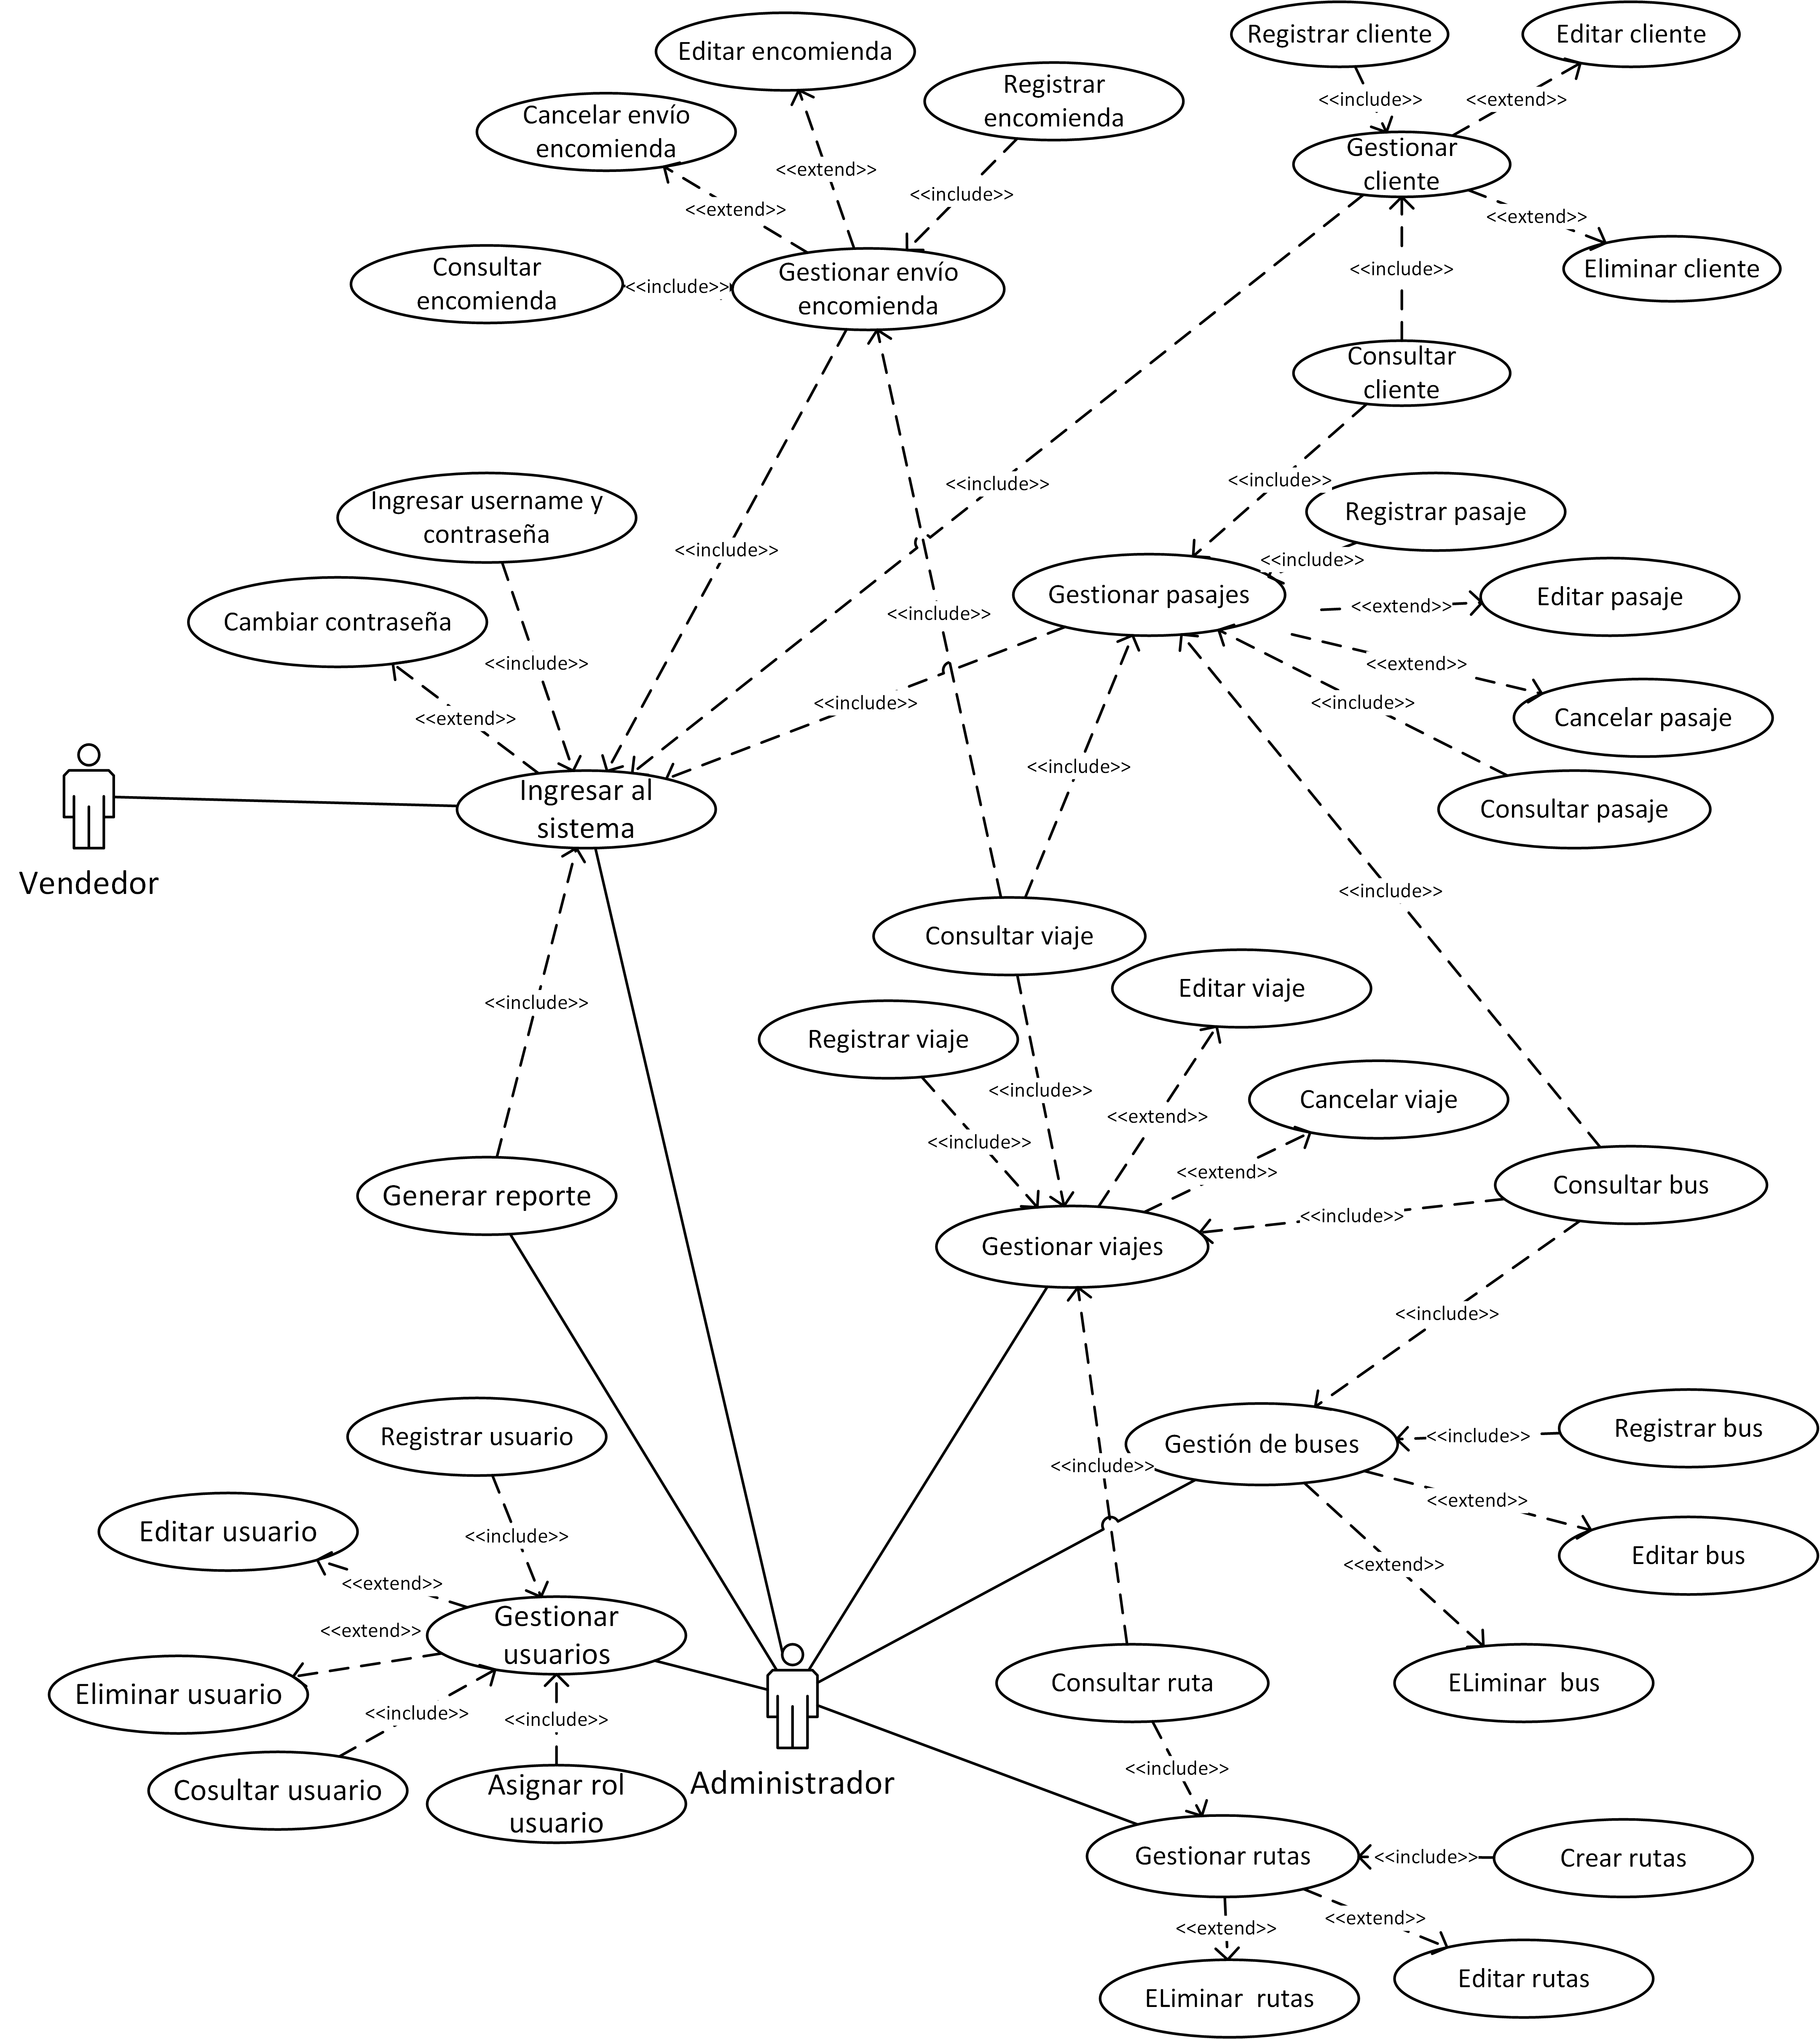
\includegraphics[width=1\textwidth]{imagenes/cap_3/casos_de_uso.png} % Inserta una imagen
		\vspace{0.3cm}
		%\caption*{\textup{\textbf{Nota}: Obtenido de https://evaluacionred-g3-2019.fandom.com/}}
		\vspace{-0.8cm}
		\label{fig:caso_uso} % Etiqueta para referencia cruzada
	\end{figure}
	
	\noindent \textbf{Especificaciones de casos de uso}
	
	El presente apartado desde la tabla \ref{tab:tabla3_2} a la tabla \ref{tab:tabla3_10} contiene la especificación detallada de los casos de uso del sistema, organizados por módulos funcionales, para cada caso se describe el alcance, los objetivos específicos y las interacciones necesarias para completar las funcionalidades requeridas, proporcionando una visión clara del comportamiento esperado.
	
	\begingroup
	\onehalfspacing
	
	\begin{longtable}{m{4cm} m{10.5cm}}
		\caption[Especificación de casos de uso: Autenticación del usuario]{\newline Especificación de casos de uso: Autenticación del usuario} \label{tab:tabla3_2}\\
		\toprule
		\textbf{Caso de Uso} & Autenticación del usuario \\
		\midrule
		\endfirsthead
		
		% \toprule
		\textbf{Caso de Uso} & Autenticación del usuario \\
		\midrule
		\endhead
		
		%\midrule
		%\multicolumn{2}{r}{\textit{Continúa en la siguiente página}} \\
		%\midrule
		%\endfoot
		
		\bottomrule
		\endlastfoot
		
		% Aquí se colocan las filas de la tabla, por ejemplo:
		\textbf{Descripción} & La página de autenticación de usuarios permite al administrador y al personal de atención al cliente acceder al sistema y realizar funciones de cada usuario \\ \hline
		\textbf{Actores} & Administrador, Personal de atención al cliente \\ \hline
		\textbf{Precondiciones} & El usuario debe contar con un nombre de usuario y una contraseña asignados previamente para poder acceder a las opciones del sistema web. \\ \hline
		\textbf{Secuencia Normal} & 
			El usuario y la contraseña son validados en la base de datos.
			
			Se verifica en la base de datos el tipo de usuario que se ha autenticado y se lo dirige a las opciones pertinentes.
			
			Se visualizan las opciones que tiene cada usuario. \\ \hline
		\textbf{Postcondiciones} & Los datos del usuario se mantienen mientras su sesión esté abierta después de que se ha autenticado en el sistema.\\ \hline
		\textbf{Excepciones} & Si el usuario y la contraseña no existen en la base de datos o si la contraseña no corresponde al usuario, se muestra una notificación de error solicitando nuevamente los datos. \\		
	\end{longtable}
	
	\endgroup 
	\vspace{-6pt}  % O el valor que necesites para ajustar
	% Nota personalizada fuera de `\caption*{}`
	% \textbf{Nota}: Esta es la nota de la tabla, explicando datos relevantes.
	
	\begingroup
	\onehalfspacing
	
	\begin{longtable}{m{4cm} m{10.5cm}}
		\caption[Especificación de casos de uso: Gestionar bus]{\newline Especificación de casos de uso: Gestionar bus} \label{tab:tabla3_3}\\
		\toprule
		\textbf{Caso de Uso} & Gestionar bus \\
		\midrule
		\endfirsthead
		
		\toprule
		\textbf{Caso de Uso} & Gestionar bus \\
		% \midrule
		\endhead
		
		%\midrule
		%\multicolumn{2}{r}{\textit{Continúa en la siguiente página}} \\
		%\midrule
		%\endfoot
		
		\bottomrule
		\endlastfoot
		
		% Aquí se colocan las filas de la tabla, por ejemplo:
		\textbf{Descripción} & Este caso de uso hace referencia registro de los datos de un bus. \\ \hline
		\textbf{Actores} & Administrador \\ \hline
		\textbf{Precondiciones} & El administrador debe acceder al sistema con su usuario y contraseña. \\ \hline
		\textbf{Secuencia Normal} & El administrador debe elegir la opción “Configurar Bus” del ítem “Configurar”.
		
		El administrador debe consultar la existencia del bus a registrar.
		
		El administrador debe completar la placa del bus, la capacidad de personas, modelo, y año.
		
		El administrador guarda el registro realizado.
		
		El administrador podrá editar los datos del registro y eliminar el registro realizado. \\ \hline
		\textbf{Postcondiciones} & Ninguna.\\ \hline
		\textbf{Excepciones} & Si el usuario y la contraseña no existen en la base de datos o si la contraseña no corresponde al usuario, se muestra una notificación de error solicitando nuevamente los datos.
		
		De no completar los datos en los registros, se mostrará un mensaje mencionando qué datos están vacíos y cuáles no han sido seleccionados. \\
	\end{longtable}
	
	\endgroup 
	\vspace{-6pt}  % O el valor que necesites para ajustar
	% Nota personalizada fuera de `\caption*{}`
	% \textbf{Nota}: Esta es la nota de la tabla, explicando datos relevantes.
	
	\begingroup
	\onehalfspacing
	
	\begin{longtable}{m{4cm} m{10.5cm}}
		\caption[Especificación de casos de uso: Gestionar rutas]{\newline Especificación de casos de uso: Gestionar rutas} \label{tab:tabla3_4}\\
		\toprule
		\textbf{Caso de Uso} & Gestionar rutas \\
		\midrule
		\endfirsthead
		
		\toprule
		\textbf{Caso de Uso} & Gestionar rutas \\
		% \midrule
		\endhead
		
		%\midrule
		%\multicolumn{2}{r}{\textit{Continúa en la siguiente página}} \\
		%\midrule
		%\endfoot
		
		\bottomrule
		\endlastfoot
		
		% Aquí se colocan las filas de la tabla, por ejemplo:
		\textbf{Descripción} & Este caso de uso hace referencia al registro de los lugares de origen y destino. \\ \hline
		\textbf{Actores} & Administrador \\ \hline
		\textbf{Precondiciones} & El administrador debe acceder al sistema con su usuario y contraseña. \\ \hline
		\textbf{Secuencia Normal} & El administrador debe elegir la opción “Registrar rutas” del ítem “Registro”.
		
		El administrador debe consultar la existencia de las rutas de origen y de destino a registrar.
		
		El administrador debe completar los datos del lugar de origen como el nombre de la ciudad. Por defecto el estado muestra como activo. De igual manera el administrador deberá completar los mismos datos para el lugar de destino.
		
		El administrador guarda el registro realizado.
		
		El administrador podrá editar los datos del registro, eliminar el registro realizado y cambiar el estado del registro. \\ \hline
		\textbf{Postcondiciones} & Ninguna.\\ \hline
		\textbf{Excepciones} & Si el usuario y la contraseña no existen en la base de datos o si la contraseña no corresponde al usuario, se muestra una notificación de error solicitando nuevamente los datos.
		
		De no completar los datos en los registros, se mostrará un mensaje mencionando qué datos están vacíos y cuáles no han sido seleccionados.
		
	\end{longtable}
	
	\endgroup 
	\vspace{-6pt}  % O el valor que necesites para ajustar
	% Nota personalizada fuera de `\caption*{}`
	% \textbf{Nota}: Esta es la nota de la tabla, explicando datos relevantes.	
	
	\begingroup
	\onehalfspacing
	
	\begin{longtable}{m{4cm} m{10.5cm}}
		\caption[Especificación de casos de uso: Gestionar viajes]{\newline Especificación de casos de uso: Gestionar viajes} \label{tab:tabla3_5}\\
		\toprule
		\textbf{Caso de Uso} & Gestionar viajes \\
		\midrule
		\endfirsthead
		
		\toprule
		\textbf{Caso de Uso} & Gestionar viajes \\
		% \midrule
		\endhead
		
		%\midrule
		%\multicolumn{2}{r}{\textit{Continúa en la siguiente página}} \\
		%\midrule
		%\endfoot
		
		\bottomrule
		\endlastfoot
		
		% Aquí se colocan las filas de la tabla, por ejemplo:
		\textbf{Descripción} & Este caso de uso hace referencia a la programación de los viajes con sus fechas respectivas para cada uno, se asignará un viaje a un bus y por defecto se indicarán los lugares de origen y destino. Tendrá un estado de viaje. \\ \hline
		\textbf{Actores} & Administrador \\ \hline
		\textbf{Precondiciones} & El administrador debe acceder al sistema con su usuario y contraseña. \\ \hline
		\textbf{Secuencia Normal} & El administrador debe elegir la opción “Registrar viajes” del ítem “Registro”.
		
		El administrador debe consultar el bus que realizará un viaje.
		
		El sistema muestra el lugar de ubicación del bus y por defecto lo asigna al campo de ciudad de origen. También se completan los campos de capacidad de personas y límite de carga.
		
		El administrador debe completar la ciudad de destino, debe programar la fecha de salida y de llegada del viaje. Debe elegir un estado del viaje que por defecto el sistema muestra como PENDIENTE.
		
		El administrador guarda el registro realizado.
		
		El administrador podrá editar los datos del registro y eliminar el registro realizado. \\ \hline
		\textbf{Postcondiciones} & Ninguna.\\ \hline
		\textbf{Excepciones} & Si el usuario y la contraseña no existen en la base de datos o si la contraseña no corresponde al usuario, se muestra una notificación de error solicitando nuevamente los datos.
		
		De no completar los datos en los registros, se mostrará un mensaje mencionando qué datos están vacíos y cuáles no han sido seleccionados.
		
	\end{longtable}
	
	\endgroup 
	\vspace{-6pt}  % O el valor que necesites para ajustar
	% Nota personalizada fuera de `\caption*{}`
	% \textbf{Nota}: Esta es la nota de la tabla, explicando datos relevantes.
	
	\begingroup
	\onehalfspacing
	
	\begin{longtable}{m{4cm} m{10.5cm}}
		\caption[Especificación de casos de uso: Gestionar pasaje]{\newline Especificación de casos de uso: Gestionar pasaje} \label{tab:tabla3_6}\\
		\toprule
		\textbf{Caso de Uso} & Gestionar pasaje \\
		\midrule
		\endfirsthead
		
		\toprule
		\textbf{Caso de Uso} & Gestionar pasaje \\
		% \midrule
		\endhead
		
		%\midrule
		%\multicolumn{2}{r}{\textit{Continúa en la siguiente página}} \\
		%\midrule
		%\endfoot
		
		\bottomrule
		\endlastfoot
		
		% Aquí se colocan las filas de la tabla, por ejemplo:
		\textbf{Descripción} & Este caso de uso hace referencia a la venta de pasajes para los buses. \\ \hline
		\textbf{Actores} & Personal de atención al cliente \\ \hline
		\textbf{Precondiciones} & El recepcionista debe acceder al sistema con su usuario y contraseña. \\ \hline
		\textbf{Secuencia Normal} & El recepcionista debe elegir la opción “Ventas” del ítem “Pasajes”.
		
		El recepcionista consulta el día del viaje, el sistema mostrará la lista de viajes programados según la fecha actual del sistema. Por defecto se completan los datos de la ciudad
		de origen y de destino y el bus programado.
		
		El recepcionista debe consultar un asientos libres en el buses disponibles.
		
		El recepcionista debe consultar una ruta de destino del pasajero.
		
		El recepcionista consulta de la existencia del cliente; si existe se obtienen los datos y se completan en los campos vacíos, si no existe procede a registrar los datos de los clientes.
		
		Debe existir un contador regresivo según de cada registro de pasajeros y del aforo de la embarcación.
		
		Por defecto se completan los datos en los demás campos según el registro de los datos de las personas, el sistema consulta, calcula el monto del pago y completa los campos.
		
		El recepcionista guarda el registro.
		
		Se imprime el boleto del pasaje con los datos del pasajero, el destino, el monto de pago, el tipo de pasaje y con un número de ticket.
		
		El recepcionista también podrá editar los datos del registro del pasaje y cancelar el registro. \\ \hline
		\textbf{Postcondiciones} & Ninguna.\\ \hline
		\textbf{Excepciones} & Si el usuario y la contraseña no existen en la base de datos o si la contraseña no corresponde al usuario, se muestra una notificación de error solicitando nuevamente los datos.
		
		De no completar los datos en los registros, se mostrará un mensaje mencionando qué datos están vacíos y cuáles no han sido seleccionados.
		
		De sobrepasar el límite de aforo del bus permitido, el sistema no permitirá más registros. \\
	\end{longtable}
	
	\endgroup 
	\vspace{-6pt}  % O el valor que necesites para ajustar
	% Nota personalizada fuera de `\caption*{}`
	% \textbf{Nota}: Esta es la nota de la tabla, explicando datos relevantes.
	
	\begingroup
	\onehalfspacing
	
	\begin{longtable}{m{4cm} m{10.5cm}}
		\caption[Especificación de casos de uso: Gestionar reserva de pasaje]{\newline Especificación de casos de uso: Gestionar reserva de pasaje} \label{tab:tabla3_7}\\
		\toprule
		\textbf{Caso de Uso} & Gestionar reserva de pasaje \\
		\midrule
		\endfirsthead
		
		\toprule
		\textbf{Caso de Uso} & Gestionar reserva de pasaje \\
		% \midrule
		\endhead
		
		%\midrule
		%\multicolumn{2}{r}{\textit{Continúa en la siguiente página}} \\
		%\midrule
		%\endfoot
		
		\bottomrule
		\endlastfoot
		
		% Aquí se colocan las filas de la tabla, por ejemplo:
		\textbf{Descripción} & Caso de uso orientado a gestionar las reservas de pasajes en el sistema de gestión de ventas de pasajes de la empresa. \\ \hline
		\textbf{Actores} & Personal de atención al cliente \\ \hline
		\textbf{Precondiciones} & El recepcionista debe acceder al sistema con su usuario y contraseña. \\ \hline
		\textbf{Secuencia Normal} & El recepcionista debe elegir la opción “Reservas” del ítem
		“Pasajes”.
		
		El recepcionista debe consultar las salidas programadas para un viaje, el sistema mostrará la lista de salidas según la fecha actual del sistema. Por defecto se completan los datos de la ciudad de origen y de destino y el bus programado.
		
		El recepcionista debe elegir un número de asiento para continuar con el registro.
		
		El recepcionista realiza una consulta de la existencia del cliente; si existe se obtienen los datos y se completan en los campos vacíos, si no existe procede a registrar los datos de los clientes.
			
		Por defecto se completan los datos en los demás campos según el registro de los datos de los clientes, el sistema consulta, calcula el monto del pago y completa los campos.
		
		El sistema obtendrá un código de reserva con los parámetros según la ciudad de origen, la ciudad de destino y un número correlativo de acuerdo a los registros progresivos.
		
		El sistema por defecto muestra el estado de la reserva como PENDIENTE, la reserva tendrá 3 horas de validez, pasado la hora se eliminará la reserva.
		
		El recepcionista guarda el registro realizado. 
		
		El recepcionista podrá editar los datos del registro y eliminar la reserva realizada. \\ \hline
		
		\textbf{Postcondiciones} & Ninguna.\\ \hline
		\textbf{Excepciones} & Si el usuario y la contraseña no existen en la base de datos o si la contraseña no corresponde al usuario, se muestra una notificación de error solicitando nuevamente los datos.
		
		De no completar los datos de la reserva, se mostrará un mensaje mencionando qué datos están vacíos y cuáles no han sido seleccionados.
		
		De sobrepasar el límite de aforo del bus permitido, el sistema no permitirá más registros. \\ 
		
	\end{longtable}
	
	\endgroup 
	\vspace{-6pt}  % O el valor que necesites para ajustar
	% Nota personalizada fuera de `\caption*{}`
	% \textbf{Nota}: Esta es la nota de la tabla, explicando datos relevantes.
	
	
	\begingroup
	\onehalfspacing
	
	\begin{longtable}{m{4cm} m{10.5cm}}
		\caption[Especificación de casos de uso: Gestionar encomienda]{\newline Especificación de casos de uso: Gestionar encomienda} \label{tab:tabla3_8}\\
		\toprule
		\textbf{Caso de Uso} & Gestionar encomienda \\
		\midrule
		\endfirsthead
		
		\toprule
		\textbf{Caso de Uso} & Gestionar encomienda \\
		% \midrule
		\endhead
		
		%\midrule
		%\multicolumn{2}{r}{\textit{Continúa en la siguiente página}} \\
		%\midrule
		%\endfoot
		
		\bottomrule
		\endlastfoot
		
		% Aquí se colocan las filas de la tabla, por ejemplo:
		\textbf{Descripción} & Este caso de uso hace referencia al registro de las encomiendas: se consulta el viaje programado para el día del envío, también registrar los datos del remitente y destinatario. Se debe especificar el tipo de encomienda, la cantidad y descripción de lA encomienda, el monto calculado por el personal de atención al cliente encargado del registro. \\ \hline
		\textbf{Actores} & Personal de atención al cliente \\ \hline
		\textbf{Precondiciones} & El recepcionista debe acceder al sistema con su usuario y contraseña. \\ \hline
		\textbf{Secuencia Normal} & 
		El recepcionista debe elegir la opción “Registrar encomienda” del ítem “Encomienda”.
		
		El recepcionista debe consultar el día del viaje, en el sistema muestra la lista de viajes más próximos a la fecha actual del sistema. Por defecto se completan los campos
		del lugar de origen y destino y el bus programado.
		
		El recepcionista realiza una consulta de la existencia de los clientes (remitente y destinatario); si existen se obtienen los datos y se asignan los campos vacíos, si no existe procede a registrar los datos de los clientes.
		
		El recepcionista debe registrar los datos del encargo: encomienda, correspondencia o carga. Debe seleccionar un tipo de encargo, debe llenar una descripción de la encomienda, la cantidad y el monto a pagar. El estado del encargo por defecto se guarda como “PENDIENTE”.
		
		El recepcionista debe guardar el registro realizado.
		
		El recepcionista debe imprimir el comprobante del registro del encargo.
		
		Cuando la encomienda llega a su destino y se realza al recojo del mismo, el recepcionista debe constatar que la persona que recoge sea la misma registrada en el sistema; debe actualizar el estado del encargo a “ENTREGADO” y hacer entrega de la encomienda. \\ \hline
		\textbf{Postcondiciones} & Ninguna.\\ \hline
		\textbf{Excepciones} & Si el usuario y la contraseña no existen en la base de datos o si la contraseña no corresponde al usuario, se muestra una notificación de error solicitando nuevamente los datos.
		
		De no completar los datos en los registros, se mostrará un mensaje mencionando qué datos están vacíos y cuáles no han sido seleccionados.
		
		De sobrepasar el límite de peso permitido de las cargas, el sistema rechazará el registro de más cargas
		
		De no actualizar el estado del encargo entregado, éste se mantendrá como pendiente de recoger. \\		
	\end{longtable}
	
	\endgroup 
	\vspace{-6pt}  % O el valor que necesites para ajustar
	% Nota personalizada fuera de `\caption*{}`
	% \textbf{Nota}: Esta es la nota de la tabla, explicando datos relevantes.
	
	\begingroup
	\onehalfspacing
	
	\begin{longtable}{m{4cm} m{10.5cm}}
		\caption[Especificación de casos de uso: Gestionar rol de usuario]{\newline Especificación de casos de uso: Gestionar rol de usuario} \label{tab:tabla3_9}\\
		\toprule
		\textbf{Caso de Uso} & Gestionar rol de usuario \\
		\midrule
		\endfirsthead
		
		\toprule
		\textbf{Caso de Uso} & Gestionar rol de usuario \\
		% \midrule
		\endhead
		
		%\midrule
		%\multicolumn{2}{r}{\textit{Continúa en la siguiente página}} \\
		%\midrule
		%\endfoot
		
		\bottomrule
		\endlastfoot
		
		% Aquí se colocan las filas de la tabla, por ejemplo:
		\textbf{Descripción} & Este caso de uso hace referencia al registro un rol de usuario. \\ \hline
		\textbf{Actores} & Administrador \\ \hline
		\textbf{Precondiciones} & El administrador debe acceder al sistema con su usuario y contraseña. \\ \hline
		\textbf{Secuencia Normal} & El administrador debe elegir la opción “Configurar roles” del ítem “Configurar”.
		
		El administrador debe consultar la existencia del rol a registrar.
		
		El administrador debe completar los campos de nombre del rol, registrar una descripción del rol.
		
		El administrador debe seleccionar los accesos que tendrá el rol al sistema.
		
		El administrador guarda el registro realizado.
		
		El administrador podrá editar los datos del registro y eliminar el registro realizado. \\ \hline
		\textbf{Postcondiciones} & Ninguna.\\ \hline
		\textbf{Excepciones} & Si el usuario y la contraseña no existen en la base de datos o si la contraseña no corresponde al usuario, se muestra una notificación de error solicitando nuevamente los datos.
		
		De no completar los datos en los registros, se mostrará un mensaje mencionando qué datos están vacíos y cuáles no han sido seleccionados. \\		
	\end{longtable}
	
	\endgroup 
	\vspace{-6pt}  % O el valor que necesites para ajustar
	% Nota personalizada fuera de `\caption*{}`
	% \textbf{Nota}: Esta es la nota de la tabla, explicando datos relevantes.
	
	\begingroup
	\onehalfspacing
	
	\begin{longtable}{m{4cm} m{10.5cm}}
		\caption[Especificación de casos de uso: Generar reporte]{\newline Especificación de casos de uso: Generar reporte} \label{tab:tabla3_10}\\
		\toprule
		\textbf{Caso de Uso} & Generar reporte \\
		\midrule
		\endfirsthead
		
		\toprule
		\textbf{Caso de Uso} & Generar reporte \\
		% \midrule
		\endhead
		
		%\midrule
		%\multicolumn{2}{r}{\textit{Continúa en la siguiente página}} \\
		%\midrule
		%\endfoot
		
		\bottomrule
		\endlastfoot
		
		% Aquí se colocan las filas de la tabla, por ejemplo:
		\textbf{Descripción} & Este caso de uso hace referencia al proceso de generación de reportes necesarios para la gestión administrativa de la empresa. \\ \hline
		\textbf{Actores} & Administrador, personal de atención al cliente \\ \hline
		\textbf{Precondiciones} & El administrador o personal de atención al cliente debe acceder al sistema con su usuario y contraseña. \\ \hline
		\textbf{Secuencia Normal} & El usuario puede ver dentro del sistema sólo los reportes que su perfil le permita, cabe mencionar que el perfil con todos los
		permisos u opciones es el Administrador.
		
		El usuario selecciona el reporte que desea generar.
		
		El usuario ingresa los parámetros de búsqueda antes de generar el reporte.
		
		El sistema muestra los datos del reporte.
		
		El sistema imprime el reporte seleccionado. \\ \hline
		\textbf{Postcondiciones} & Ninguna.\\ \hline
		\textbf{Excepciones} & Si el usuario y la contraseña no existen en la base de datos o si la contraseña no corresponde al usuario, se muestra una notificación de error solicitando nuevamente los datos. \\		
	\end{longtable}
	
	\endgroup 
	\vspace{-6pt}  % O el valor que necesites para ajustar
	% Nota personalizada fuera de `\caption*{}`
	% \textbf{Nota}: Esta es la nota de la tabla, explicando datos relevantes.
		
	\subsection{Especificación de requerimientos}
	En esta etapa del proyecto, se presenta la especificación detallada de los requerimientos funcionales y no funcionales identificados para el sistema. Esta sección tiene como objetivo proporcionar una descripción completa de las capacidades y restricciones que deberá cumplir la solución, estableciendo así las bases para su posterior diseño e implementación.\\
	\textbf{Requerimientos funcionales} \\		
	\textbf{RF-01:} El sistema contará con un módulo de gestión de perfiles de usuarios, distinguiendo entre administradores y empleados. \\	
	\textbf{RF-02:} El sistema permitirá la gestión de rutas y horarios de los servicios de transporte. \\	
	\textbf{RF-03:} El sistema contará con un módulo de venta y reserva de boletos para los usuarios. \\	
	\textbf{RF-04:} El sistema realizará la asignación de asientos en los vehículos de transporte. \\	
	\textbf{RF-05:} El sistema permitirá el registro y seguimiento de las encomiendas transportadas. \\	
	\textbf{RF-06:} El sistema gestionará la flota de buses, incluyendo información de los vehículos y conductores. \\	
	\textbf{RF-07:} El sistema generará reportes de ventas y otros indicadores clave del negocio.\\
	\textbf{Requerimientos no funcionales} \\	
	\textbf{RNF-01:} El sistema debe ser accesible desde múltiples dispositivos (computadoras, tablets y móviles). \\	
	\textbf{RNF-02:} Garantizar la protección de los datos de los usuarios mediante protocolos de seguridad adecuados. \\	
	\textbf{RNF-03:} Escalabilidad, capacidad de crecer para manejar aumento en usuarios y transacciones. \\	
	\textbf{RNF-04:} Mantenibilidad, arquitectura modular para facilitar actualizaciones
		
	\subsection{Validación de requerimientos}
	

	

\section{DISEÑO DEL SISTEMA Y DEL SOFTWARE}
\section{IMPLEMENTACIÓN Y PRUEBA DE UNIDAD}
\section{INTEGRACIÓN Y PRUEBA DE SISTEMA}
\section{OPERACIÓN Y MANTENIMIENTO}
